\documentclass{article}
\usepackage{graphicx}
\usepackage{xcolor}
\usepackage{geometry}
\usepackage{natbib}


\title{workshop1}
\author{Azza Algatheem \thanks{azahm@ub.edu.sa}, Andrew \thanks{Andrew@exe.edu.sa}\\
\footnotesize{Department of Mathematics, University of Bisha}}
\date{March 10 2024}






%Body
\begin{document}

\maketitle
\begin{abstract}
    This papaer represent ........
\end{abstract}



\newpage
\section{Introduction}
Text Text text Text 
Text Text text Text 
Text Text text Text 
Text Text text Text 
\section{Motivation}
Text Text text Text 
Text Text text Text 
Text Text text Text 
Text Text text Text 
\subsection{Model1}
Text Text text Text 
Text Text text Text 
Text Text text Text



\newpage
\section{figures}
\begin{figure}[h]
    \centering
   (a) 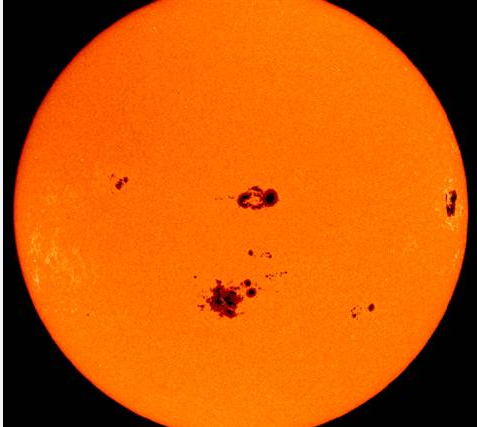
\includegraphics[scale=0.45]{sun1.png}
   (b) 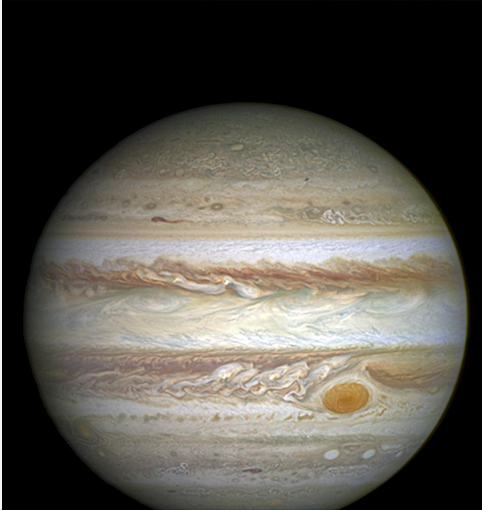
\includegraphics[scale=0.4]{jup1.png}
    \caption{this figure the sunspot....}
    \label{fig:1}
\end{figure}



Figure \ref{fig:1} shows sunspot....



\begin{table}[h]
    \centering
    \begin{tabular}{|c|c|c|}
    \hline
    Parameter& values& numbering\\
    \hline
         1&2&3  \\
         1&2&4\\ 
         \hline
    \end{tabular}
    \caption{Caption}
    \label{tab:my_label}
\end{table}

\subsection{Model2}



\section{text}
Numerical \textbf{simulations} of a two-dimensional local model are performed. The total interaction of Rossby waves without magnetic fields leads to strong zonal flows. Even a strong \textit{magnetic field effectively suppresses the generation of flows}. \cite{algatheem2023zonostrophic}We argue that the results \underline{are applicable }to understanding the effects of magnetic fields on the stability of flows and have implications for the solar tachocline.\textcolor{blue}{The benefit of this level of abstraction is that it clarifies basic aspects of instability such as how perturbation quantities grow, and how they growth rate\citep{durston2016transport} under the action of the magnetic field }.

\section{numbering}
\begin{itemize}
    \item Maths
    \item Phiscs
    \item bio
    \item chemestry
\end{itemize}

\begin{enumerate}
     \item [a]Maths
    \item [b]Phiscs
    \item [c]bio
    \item [d]chemestry
\end{enumerate}

\section{References}

\bibliography{ref}
\bibliographystyle{abbrvnat}



\end{document}

